% Chapter 4

\chapter{Chapter 4: Statistical Analysis} % Main chapter title

\label{Chapter 4} % For referencing the chapter elsewhere, use \ref{Chapter4} 

\paragraph{}
In this chapter, we will firstly calculate several metrics according to the participants' data and show the descriptive statistics. After that we will use statistical test to prove that learning does occur in both randomized and block conditions. 

%----------------------------------------------------------------------------------------
\section{Metrics Definition}
\label{sec:Metrics Definition}
\paragraph{}
As we mentioned in Section \ref{sec:Experiment Details}, we record each timestep's data of each trial, including current state, action chosen by participants, transition resulting state and reaction time. It is hard to directly analyze sequential data as in this experiment, thus we calculate several metrics for each trial, and analyze them on the trial dimension. 
\subsection{Steps}
\label{sec:Steps}
\paragraph{}
Number of steps is the most straightforward metric to measure a trial. It is obvious that the less steps participants takes, the better his policy is. This metric is named \enquote{step}. Participants' step data is shown in Fig. \ref{fig:Step Participants}. 

\begin{figure}[ht]
\centering
\subfigure[Randomized Condition]{
\begin{minipage}[t]{0.48\textwidth}
\centering
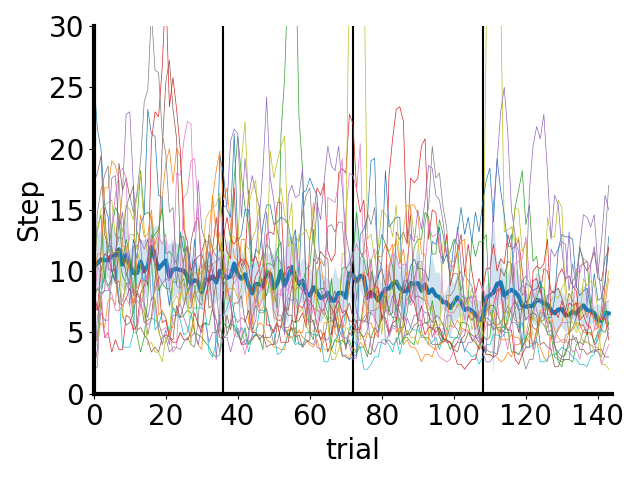
\includegraphics[width=\textwidth]{Figures/steps_randomized_participants}
\end{minipage}
}
\subfigure[Block Condition]{
\begin{minipage}[t]{0.48\textwidth}
\centering
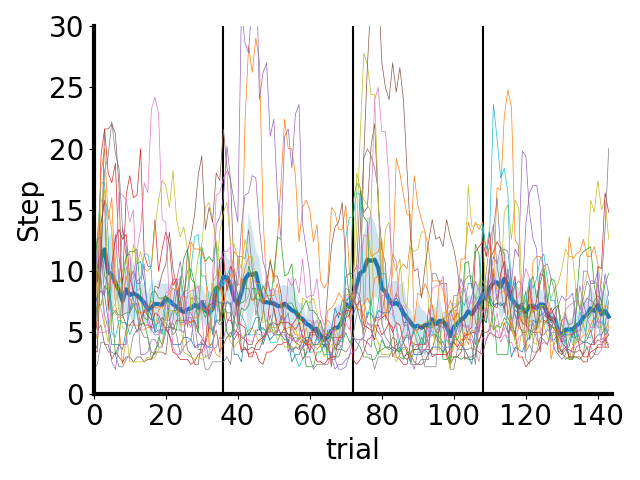
\includegraphics[width=\textwidth]{Figures/steps_block_participants}
\end{minipage}
}
\decoRule
\caption[Step data of participants]{Step data of participants in (a) randomized condition (b) block condition. The thick blue line is the mean of all participants (blue shadow indicating standard error), while the thin colorful lines are data of each participant. Vertical lines on 36, 72, 108 indicate block separation. }
\label{fig:Step Participants}
\end{figure}



\subsection{Reaction Time and Normalized Reaction Time}
\label{sec:Reaction Time and Normalized Reaction Time}
\paragraph{}
The reaction time of each timestep is recorded in data. Hence, we could sum all the reaction time of all the timesteps in one trial to represent participants' overall decision making time in a single trial. This metric is named \enquote{Reaction Time}. Participant's reaction time data is shown in Fig. \ref{fig:Reaction Time Participants}. 

\begin{figure}[ht]
\centering
\subfigure[Randomized Condition]{
\begin{minipage}[t]{0.48\textwidth}
\centering
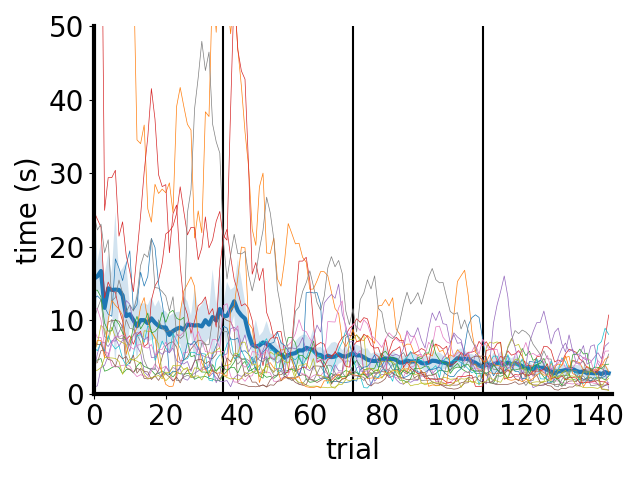
\includegraphics[width=\textwidth]{Figures/time_randomized_participants}
\end{minipage}
}
\subfigure[Block Condition]{
\begin{minipage}[t]{0.48\textwidth}
\centering
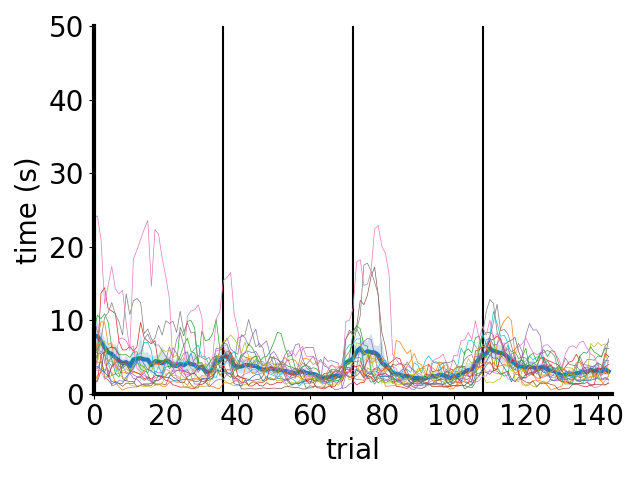
\includegraphics[width=\textwidth]{Figures/time_block_participants}
\end{minipage}
}
\decoRule
\caption[Reaction time data of participants]{Reaction time data of participants in (a) randomized condition (b) block condition. The thick blue line is the mean of all participants (blue shadow indicating standard error), while the thin colorful lines are data of each participant. Vertical lines on 36, 72, 108 indicate block separation. }
\label{fig:Reaction Time Participants}
\end{figure}

\paragraph{}
It is obvious that the \enquote{Reaction Time} metrics is strongly influenced by \enquote{Step} because of the sum operation. Thus, we create a new metric named \enquote{Normalized Reaction Time} to decrease the influence of \enquote{Step} by dividing \enquote{Reaction Time} with \enquote{Steps}. Fig \ref{fig:Normalized Reaction Time Participants} shows \enquote{Normalized Reaction Time} in participants. 

\begin{figure}[ht]
\centering
\subfigure[Randomized Condition]{
\begin{minipage}[t]{0.48\textwidth}
\centering
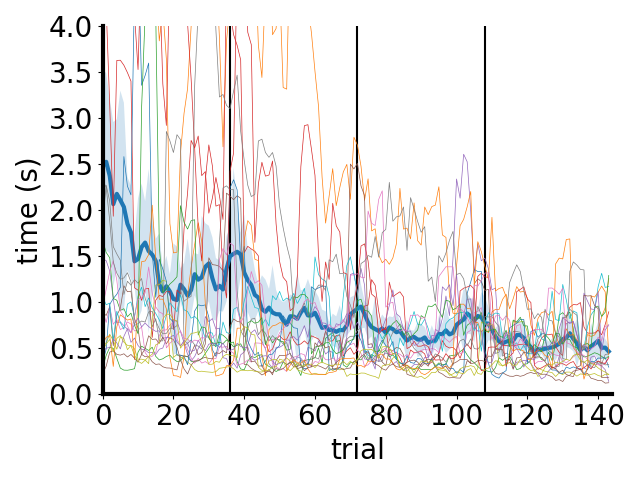
\includegraphics[width=\textwidth]{Figures/normalized_time_randomized_participants}
\end{minipage}
}
\subfigure[Block Condition]{
\begin{minipage}[t]{0.48\textwidth}
\centering
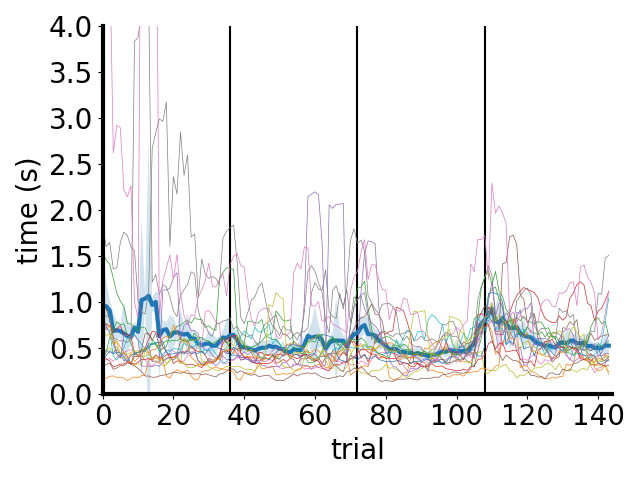
\includegraphics[width=\textwidth]{Figures/normalized_time_block_participants}
\end{minipage}
}
\decoRule
\caption[Normalized Reaction time data of participants]{Normalized Reaction time data of participants in (a) randomized condition (b) block condition. The thick blue line is the mean of all participants (blue shadow indicating standard error), while the thin colorful lines are data of each participant. Vertical lines on 36, 72, 108 indicate block separation. }
\label{fig:Normalized Reaction Time Participants}
\end{figure}


\subsection{Optimal Percentage}
\label{sec:Optimal Percentage}
\paragraph{}
All three metrics mentioned above are all straightforward from raw data. But we are most interested in how participants learn to play this task well. For this purpose, we defined several Optimal-related metrics to indicate how participants learn this task step by step. 
\paragraph{}
First we need to define \enquote{optimal}. At each state the participant is in, there exists an optimal action choose. For instance, if the goal is \emph{B}, the optimal action in \emph{A}, \emph{D}, \emph{F}, \emph{C} will all be the one whose primary consequence is \emph{E}, while the optimal action in \emph{E} is the one whose primary consequence is \emph{B}. This action is called \enquote{optimal action}. 
\paragraph{}
Thus, we could calculate whether at each timestep the participant choose the optimal action. Then we are able to calculate the optimal action percentage in each trial, making it a trial metric. This metric is called \enquote{Optimal Percentage} and its trend with trial is shown in Fig. \ref{fig:Optimal Percentage Participants}. 

% TODO increase figure axis font and thickness of axis
\begin{figure}[ht]
\centering
\subfigure[Randomized Condition]{
\begin{minipage}[t]{0.48\textwidth}
\centering
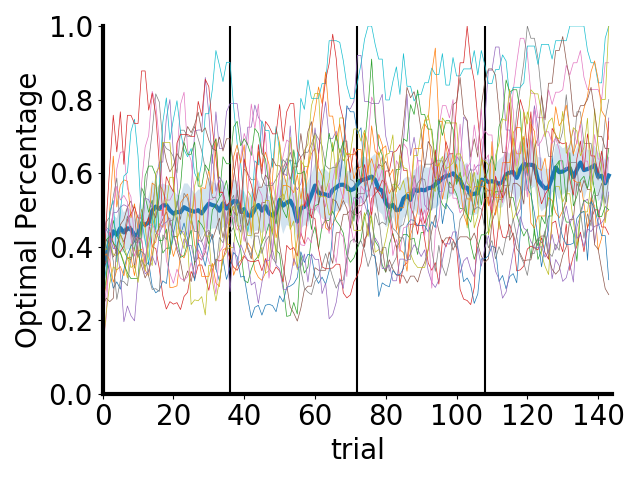
\includegraphics[width=\textwidth]{Figures/optimal_randomized_participants}
\end{minipage}
}
\subfigure[Block Condition]{
\begin{minipage}[t]{0.48\textwidth}
\centering
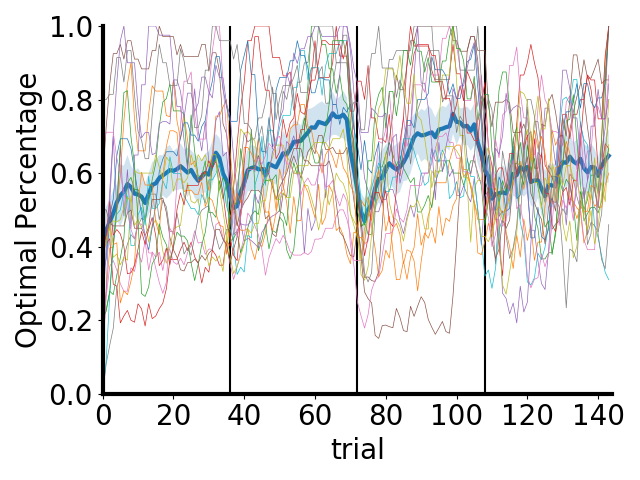
\includegraphics[width=\textwidth]{Figures/optimal_block_participants}
\end{minipage}
}
\decoRule
\caption[Optimal Percentage data of participants]{Optimal Percentage data of participants in (a) randomized condition (b) block condition. The thick blue line is the mean of all participants (blue shadow indicating standard error), while the thin colorful lines are data of each participant. Vertical lines on 36, 72, 108 indicate block separation. }
\label{fig:Optimal Percentage Participants}
\end{figure}

\paragraph{}
In order to examine participants' learning more precisely, we divide the state into three categories: \enquote{inner}, \enquote{outer}, \enquote{last}. For each trial with a end state \emph{X}, the \enquote{last} category includes only the one that can directly move to end state \emph{X}. For instance, if the end state is \emph{B}, then the \enquote{last} category includes only \emph{E} (the environment structure can be found in Fig. \ref{fig:Environment Structure}). The \enquote{inner} category includes two of three inner states \emph{D}, \emph{E}, \emph{F} except the one included in the \enquote{last} category, which in this example means the \enquote{inner} category includes \emph{D} and \emph{F}. Finally the \enquote{outer} category includes two of three outer states \emph{A}, \emph{B}, \emph{C} except the end state, which in this instance means \emph{A} and \emph{C}. Optimal Percentage in three state categories are named as \enquote{Inner Optimal Percentage}, \enquote{Outer Optimal Percentage} and \enquote{Last Optimal Percentage}. Participants' data on these three metrics are shown in Fig. \ref{fig:Inner Optimal Percentage Participants}, Fig. \ref{fig:Outer Optimal Percentage Participants} and Fig. \ref{fig:Last Optimal Percentage Participants}.

\begin{figure}[ht]
\centering
\subfigure[Randomized Condition]{
\begin{minipage}[t]{0.48\textwidth}
\centering
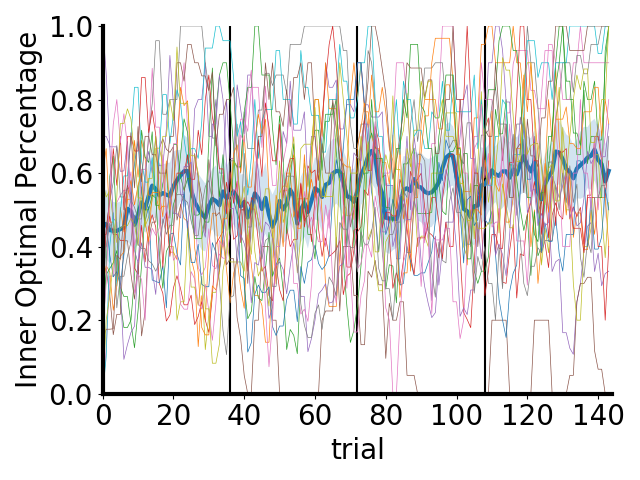
\includegraphics[width=\textwidth]{Figures/optimal_inner_randomized_participants}
\end{minipage}
}
\subfigure[Block Condition]{
\begin{minipage}[t]{0.48\textwidth}
\centering
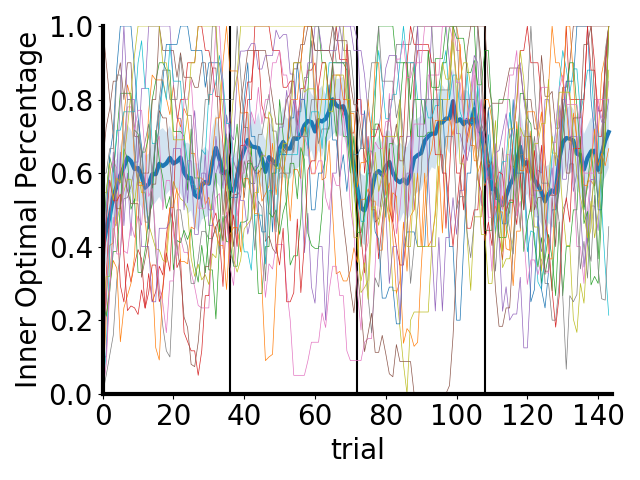
\includegraphics[width=\textwidth]{Figures/optimal_inner_block_participants}
\end{minipage}
}
\decoRule
\caption[Inner Optimal Percentage data of participants]{Inner Optimal Percentage data of participants in (a) randomized condition (b) block condition. The thick blue line is the mean of all participants (blue shadow indicating standard error), while the thin colorful lines are data of each participant. Vertical lines on 36, 72, 108 indicate block separation. }
\label{fig:Inner Optimal Percentage Participants}
\end{figure}

\begin{figure}[ht]
\centering
\subfigure[Randomized Condition]{
\begin{minipage}[t]{0.48\textwidth}
\centering
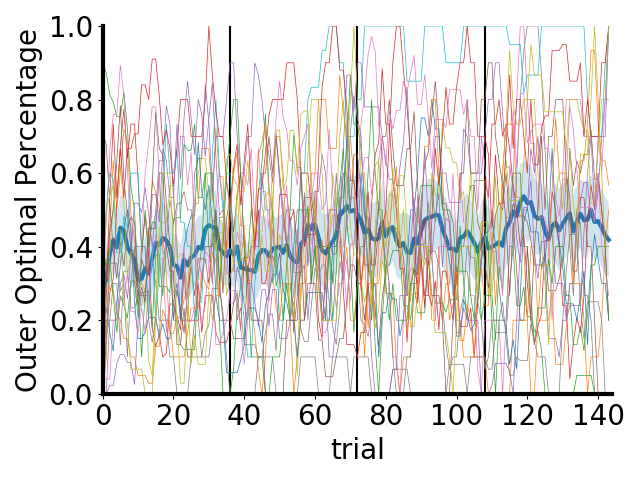
\includegraphics[width=\textwidth]{Figures/optimal_outer_randomized_participants}
\end{minipage}
}
\subfigure[Block Condition]{
\begin{minipage}[t]{0.48\textwidth}
\centering
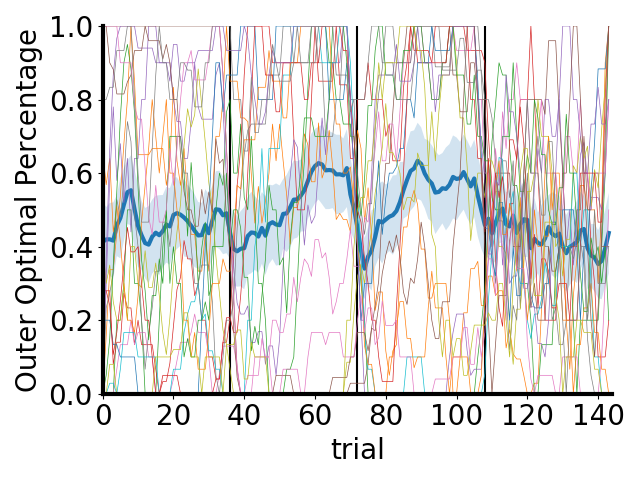
\includegraphics[width=\textwidth]{Figures/optimal_outer_block_participants}
\end{minipage}
}
\decoRule
\caption[Outer Optimal Percentage data of participants]{Outer Optimal Percentage data of participants in (a) randomized condition (b) block condition. The thick blue line is the mean of all participants (blue shadow indicating standard error), while the thin colorful lines are data of each participant. Vertical lines on 36, 72, 108 indicate block separation. }
\label{fig:Outer Optimal Percentage Participants}
\end{figure}

\begin{figure}[ht]
\centering
\subfigure[Randomized Condition]{
\begin{minipage}[t]{0.48\textwidth}
\centering
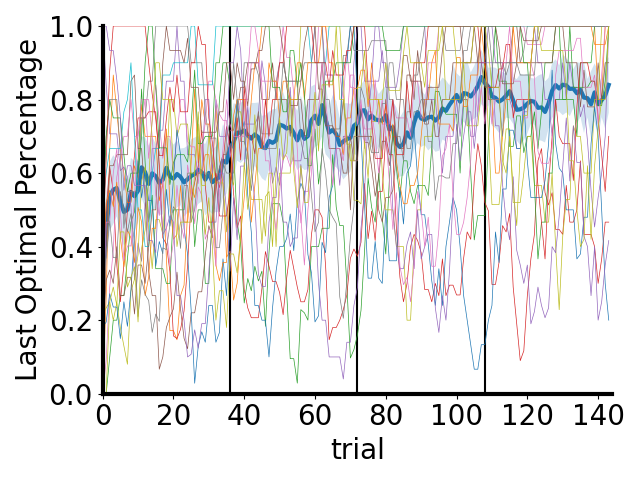
\includegraphics[width=\textwidth]{Figures/optimal_last_randomized_participants}
\end{minipage}
}
\subfigure[Block Condition]{
\begin{minipage}[t]{0.48\textwidth}
\centering
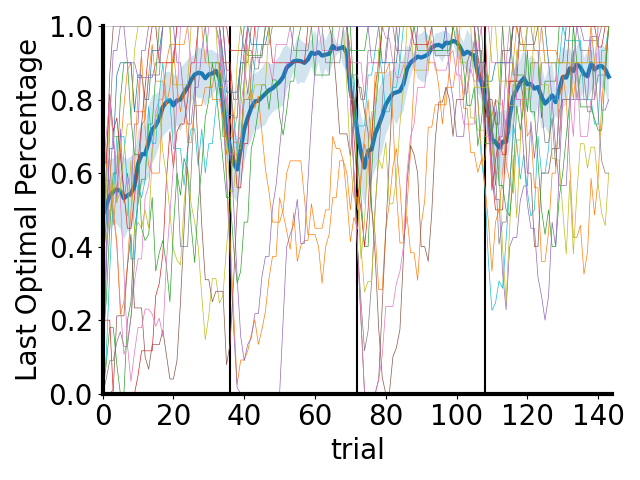
\includegraphics[width=\textwidth]{Figures/optimal_last_block_participants}
\end{minipage}
}
\decoRule
\caption[Last Optimal Percentage data of participants]{Last Optimal Percentage data of participants in (a) randomized condition (b) block condition. The thick blue line is the mean of all participants (blue shadow indicating standard error), while the thin colorful lines are data of each participant. Vertical lines on 36, 72, 108 indicate block separation. }
\label{fig:Last Optimal Percentage Participants}
\end{figure}

\paragraph{}
The advantage of \enquote{Optimal Percentage} over \enquote{Step} is that it will not be influenced by the stochasticity of the transition (action stochastic consequence), while \enquote{Step} is strongly influenced by the transition randomness even if all the actions chosen by participants are optimal. What's more, \enquote{Optimal Percentage} is a variable between 0 and 1 while \enquote{Step} does not have an upper bound, making \enquote{Optimal Percentage} metric having better statistical properties. 
\paragraph{}
The reason why we further divide \enquote{Optimal Percentage} into three categories is that we assume participants may take different learning process for each different states. For example, it is obvious that \enquote{last} category is the most simple to learn. In the meantime, it seems that participants learn \enquote{inner} category much better than \enquote{outer} category. In this way, we may divide participants' learning in three different kinds of states. 
\paragraph{}
All 7 metrics are summarized in Table \ref{table:All Metrics}, and the last column indicates whether or not it can be reflected in model simulation in Section \ref{sec:Model Simulation}. 

\begin{table}
\caption{All Metrics in Data Analysis}
\label{table:All Metrics}
\centering
\begin{tabular}{l c c}
\toprule
\tabhead{Metric Name}& \tabhead{Bound} & \tabhead{Simulation Reflected} \\
\midrule
Step & [2, Inf) & ${\surd}$ \\
Reaction Time & (0, Inf) & ${\times}$ \\
Normalized Reaction Time & (0, Inf) & ${\times}$ \\
Optimal Percentage & [0, 1] & ${\surd}$ \\
Inner Optimal Percentage & [0, 1] & ${\surd}$ \\
Outer Optimal Percentage & [0, 1] & ${\surd}$ \\
Last Optimal Percentage & [0, 1] & ${\surd}$ \\
\bottomrule\\
\end{tabular}
\end{table}
%----------------------------------------------------------------------------------------



%----------------------------------------------------------------------------------------
\section{Metrics Under Randomized Condition}
\label{sec:Metrics Under Randomized Condition}
\paragraph{}
In this section, we will analyze the learning of participants in randomized condition. We built a linear model for each metric with one independent variable: trial number. We assume that participants learn not only within-blocks but also between-blocks. The linear model $metric = {\beta}_0 + {\beta}_1 \times trial$ was fit by generalized least square method. The regression results are summarized in Table \ref{table:Linear Model for Metrics on Trial Number in Randomized condition}. 
\paragraph{}
It is clear from the result that participants do learn something about the task and their performance metrics, such as \enquote{Step}, all four \enquote{Optimal Percentage}, are getting better as trial number getting bigger. We could also see the trends in Fig. \ref{fig:Step Participants}, \ref{fig:Optimal Percentage Participants}, \ref{fig:Inner Optimal Percentage Participants}, \ref{fig:Outer Optimal Percentage Participants}, \ref{fig:Last Optimal Percentage Participants}. In the meantime, \enquote{Reaction Time} and \enquote{Normalized Reaction Time} decreases as trial number increases, indicating that participants having more confidence and making their decision quicker. It is worth noting that both \enquote{Reaction Time} and \enquote{Normalized Reaction Time} could not be reflected in the analysis of Chapter \ref{Chapter 5} in either model simulation or model fit. Therefore, it remains some space to explore in the future about these two metrics, especially when modeling uncertainty. 

\begin{table}
\caption{Linear Model for Metrics on Trial Number in Randomized condition}
\label{table:Linear Model for Metrics on Trial Number in Randomized condition}
\centering
\begin{tabular}{l c c c}
\toprule
\tabhead{Metric} & \tabhead{${\beta}_1$} & \tabhead{Significance of ${\beta}_1$} & \tabhead{${\beta}_0$} \\
\midrule
Step & -0.0299 & <.001 & 10.7862 \\
Reaction Time & -0.0726 & <.001 & 11.6328 \\
Normalized Reaction Time & -0.0090 & <.001 & 1.5710 \\
Optimal Percentage & 0.0011 & <.001 & 0.4603 \\
Inner Optimal Percentage & 0.0008 & <.001 & 0.4941 \\
Outer Optimal Percentage & 0.0007 & <.001 & 0.3692 \\
Last Optimal Percentage & 0.0020 & <.001 & 0.5662 \\
\bottomrule\\
\end{tabular}
\end{table}
%----------------------------------------------------------------------------------------




%----------------------------------------------------------------------------------------
\section{Metrics Under Block Condition}
\label{sec:Metrics Under Block Condition}
\paragraph{}
In this section, we will analyze the learning of participants in block condition. Unlike randomized condition, linear model for block condition has two independent variables: timestep and block. Note that timestep means the trial number within a block, while block represents block number. It is because in the block condition, participants will do the same task for each one of first three blocks. We assume that participants learn not only within-blocks but also between-blocks. Therefore, the linear model becomes $metric = {\beta}_0 + {\beta}_1 \times timestep + {\beta}_2 \times block$. It was fit by generalized least square method. The regression results are summarized in Table \ref{table:Linear Model for Metrics on Timestep and Block in Block condition}.

\begin{table}
\caption{Linear Model for Metrics on Timestep and Block in Block condition}
\label{table:Linear Model for Metrics on Timestep and Block in Block condition}
\centering
\begin{tabular}{l c c c c c}
\toprule
\tabhead{Metric} & \tabhead{${\beta}_1$} & \tabhead{$p$ of ${\beta}_1$} & \tabhead{${\beta}_2$} & \tabhead{$p$ of ${\beta}_2$} & \tabhead{${\beta}_0$} \\
\midrule
Step & -0.1231 & <.001 & -0.2915 & .034 & 9.8876 \\
Reaction Time & -0.0917 & <.001 & -0.2017 & .011 & 5.6542 \\
Normalized Reaction Time & -0.0068 & <.001 & -0.0289 & .071 & 0.7583 \\
Optimal Percentage & 0.0057 & <.001 & 0.0042 & .369 & 0.5137 \\
Inner Optimal Percentage & 0.0049 & <.001 & 0.0009 & .896 & 0.5477 \\
Outer Optimal Percentage & 0.0034 & .002 & -0.0106 & .172 & 0.4395 \\
Last Optimal Percentage & 0.0092 & <.001 & 0.0284 & <.001 & 0.6065 \\
\bottomrule\\
\end{tabular}
\end{table}
\paragraph{}
From the results we could tell that within-block performance is just like the randomized condition. When the timestep gets bigger, the performance gets better. We could more clearly see the trends than randomized condition in Fig. \ref{fig:Step Participants}, \ref{fig:Optimal Percentage Participants}, \ref{fig:Inner Optimal Percentage Participants}, \ref{fig:Outer Optimal Percentage Participants}, \ref{fig:Last Optimal Percentage Participants}. Just as randomized condition, \enquote{Reaction Time} and \enquote{Normalized Reaction Time} decreases as timestep increases, indicating that participants having more confidence and making their decision quicker within the block. But most importantly, there seems to show little evidence for learning between blocks. Actually, there only are \enquote{Step} ($p < .05$) and \enquote{Last Optimal Percentage} ($p < .001$) that are statistical significant. It is most likely that \enquote{Step}'s decrease is because of the increase of \enquote{Last Optimal Percentage}. The data seems to convey the message that in block condition, less is learnt between-block, indicating that each task does not assist or interfere with other tasks. We also did the same linear model of block condition for randomized condition data for comparison, and it is summarized in Table \ref{table:Linear Model for Metrics on Timestep and Block in Randomized condition}. It shows that in randomized condition, between-block learning is significant on all the performance metrics. But combining the previous analysis in \ref{sec:Metrics Under Randomized Condition}, we would conclude that the between-block learning is just the side-product of trial learning in randomized condition. 

\begin{table}
\caption{Linear Model for Metrics on Timestep and Block in Randomized condition}
\label{table:Linear Model for Metrics on Timestep and Block in Randomized condition}
\centering
\begin{tabular}{l c c c c c}
\toprule
\tabhead{Metric} & \tabhead{${\beta}_1$} & \tabhead{$p$ of ${\beta}_1$} & \tabhead{${\beta}_2$} & \tabhead{$p$ of ${\beta}_2$} & \tabhead{${\beta}_0$} \\
\midrule
Step & -0.0593 & .001 & -1.0054 & <.001 & 11.1950 \\
Reaction Time & -0.1085 & <.001 & -2.5262 & <.001 & 12.1324 \\
Normalized Reaction Time & -0.0161 & <.001 & -0.3059 & <.001 & 1.6695 \\
Optimal Percentage & 0.0011 & .021 & 0.0393 & <.001 & 0.4599 \\
Inner Optimal Percentage & 0.0005 & .460 & 0.0308 & <.001 & 0.4982 \\
Outer Optimal Percentage & 0.0008 & .288 & 0.0257 & <.001 & 0.3676 \\
Last Optimal Percentage & 0.0012 & .073 & 0.0752 & <.001 & 0.5774 \\
\bottomrule\\
\end{tabular}
\end{table}
%----------------------------------------------------------------------------------------











